\sectionframe{Label Distribution Smoothing (LDS)}
\begin{frame}{Imbalanced Categorical vs. Continuous Label Space (1/3)}
	\begin{figure}[h]
		\begin{subfigure}{0.48\textwidth}
			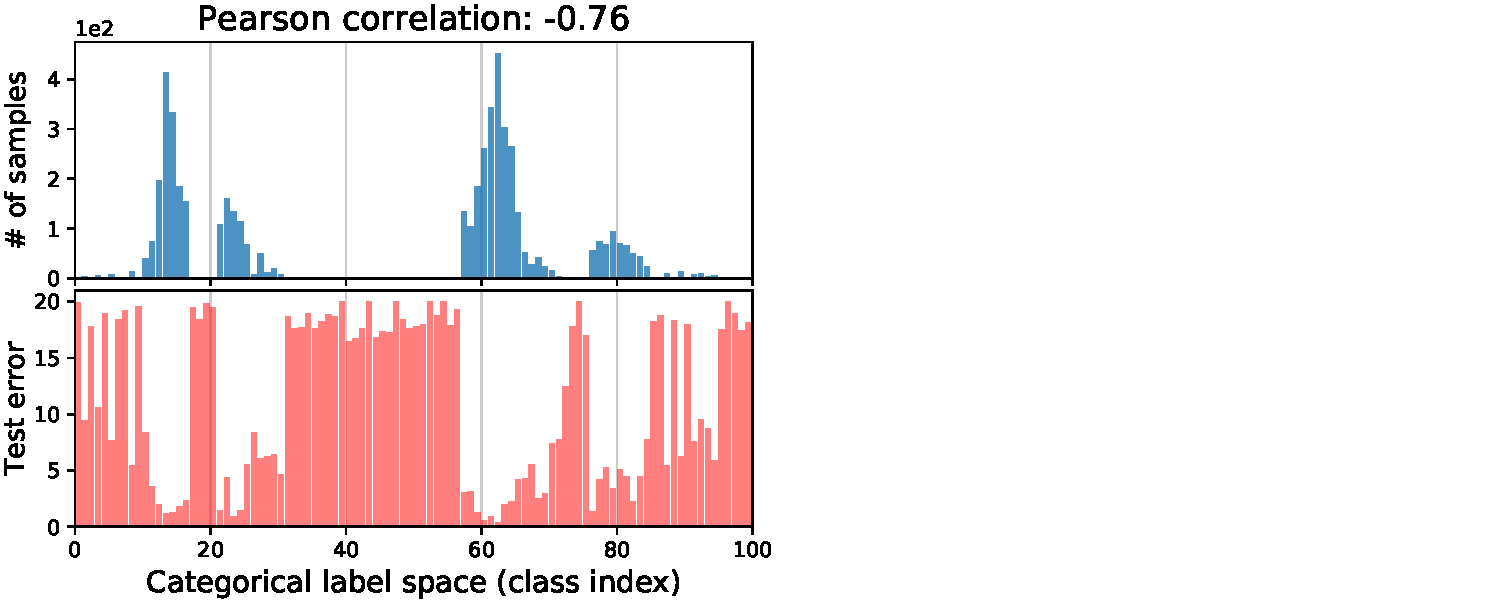
\includegraphics[width=\linewidth]{images/err_motivate_1_left.pdf}
			\caption{Classification}
		\end{subfigure}\hspace{1em}%
		\begin{subfigure}{0.44\textwidth}
			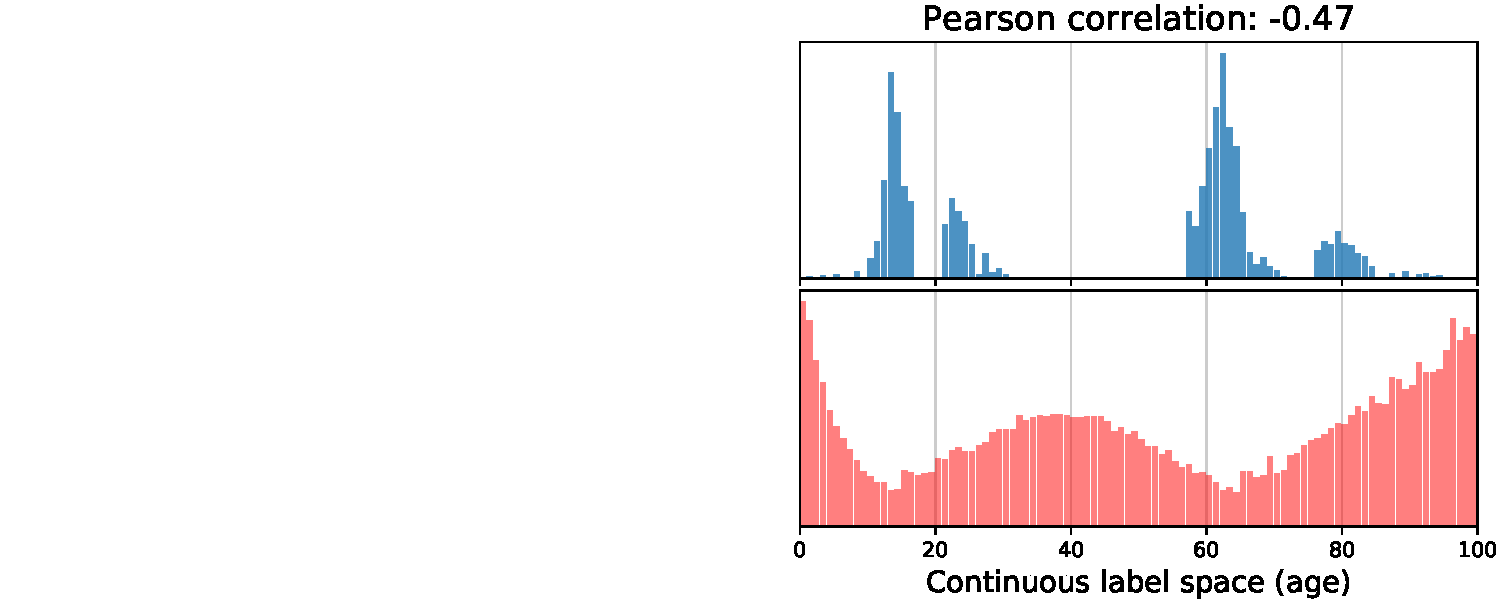
\includegraphics[width=\linewidth]{images/err_motivate_1_right.pdf}
			\caption{Regression}
		\end{subfigure}
		%\caption{}
	\end{figure}
	\footnotesize
	\vspace{-1.5em}
	\begin{columns}
		\begin{column}{0.5\textwidth}
			\begin{itemize}
				\item task: picture $\longrightarrow$ class
				\item data souce: CIFAR-100
			\end{itemize}
		\end{column}
		\begin{column}{0.5\textwidth}
			\begin{itemize}
				\item task: \\person's picture $\longrightarrow$ person's age
				\item age subrange: 0-99
				\item data souce: IMDB-WIKI
			\end{itemize}
		\end{column}
	\end{columns}
	\vspace{0.5em}
	\begin{itemize}
		\centering\item Simulated label imbalance
		\centering\item Label density distributions forced to be equal
		\centering\item Balanced test sets
	\end{itemize}
	\credit{Image}{yang2021delving}
\end{frame}

\begin{frame}{Imbalanced Categorical vs. Continuous Label Space (2/3)}
	\vspace{-2em}
	\begin{figure}[h]
		\begin{subfigure}{0.48\textwidth}
			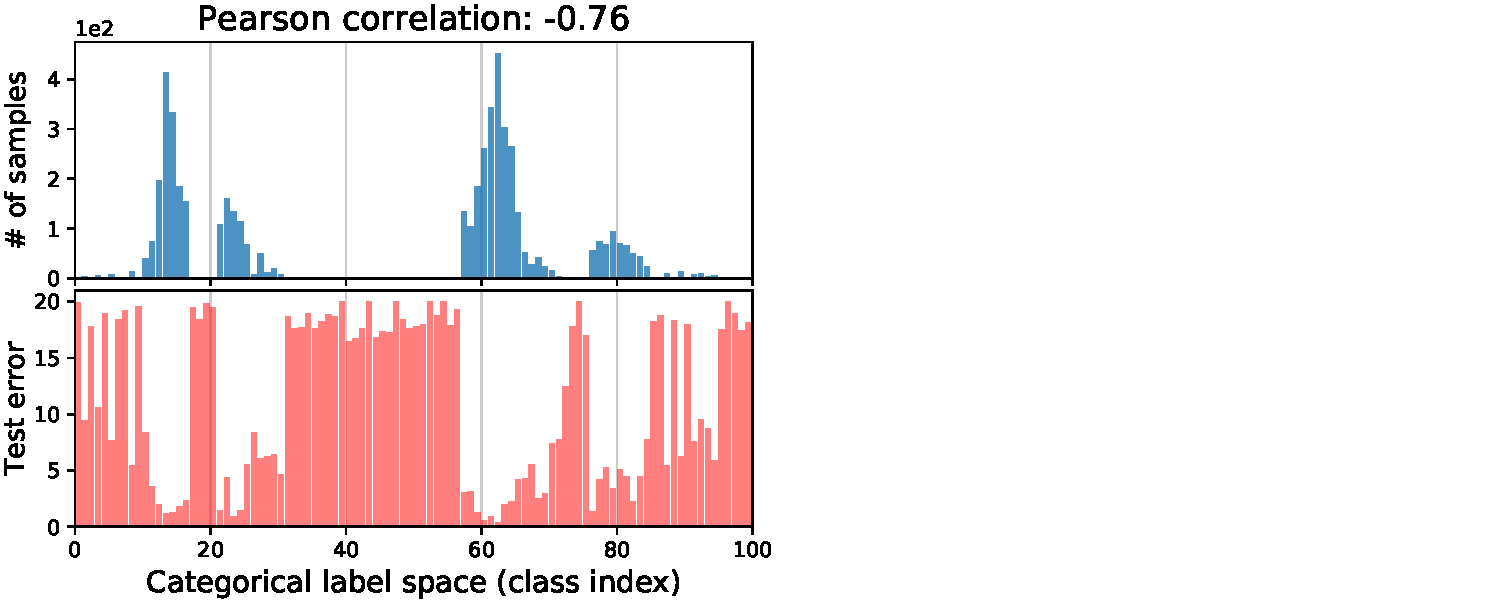
\includegraphics[width=\linewidth]{images/err_motivate_1_left.pdf}
			\caption{Classification}
		\end{subfigure}\hspace{1em}%
		\begin{subfigure}{0.44\textwidth}
			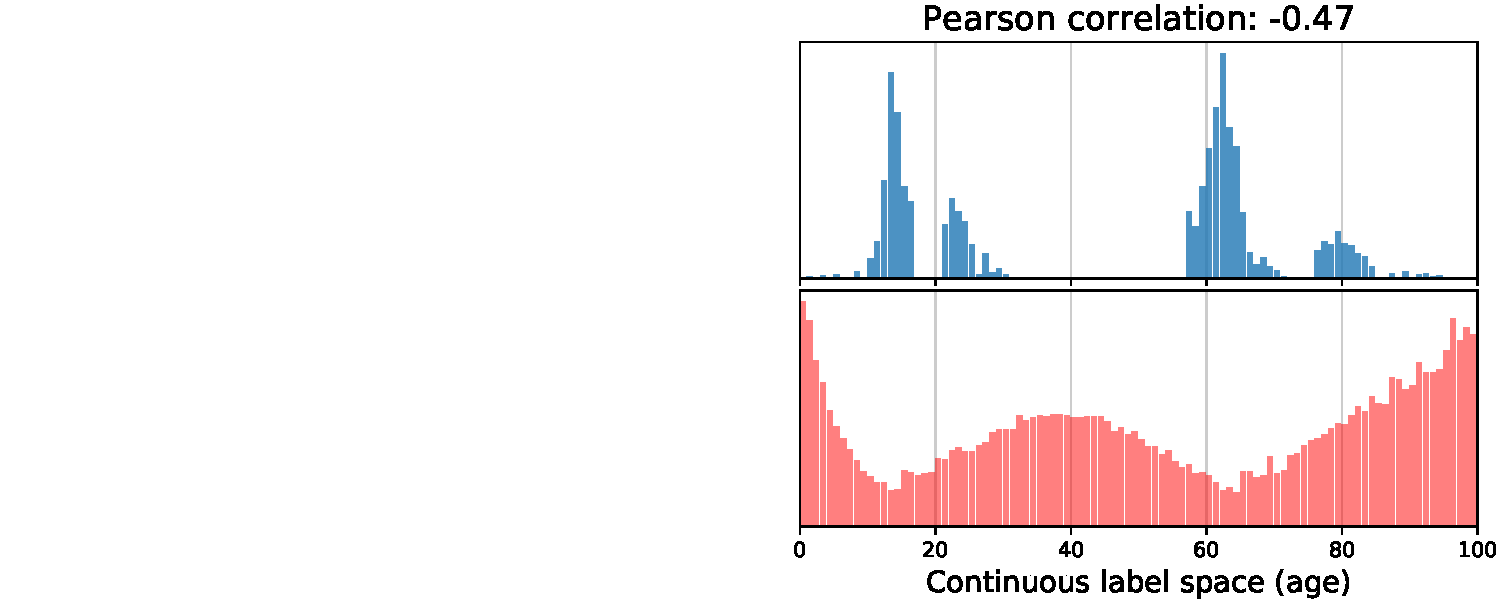
\includegraphics[width=\linewidth]{images/err_motivate_1_right.pdf}
			\caption{Regression}
		\end{subfigure}
		%\caption{}
	\end{figure}
	\footnotesize
	\vspace{-.5em}
	\begin{columns}
		\begin{column}{0.5\textwidth}
			\begin{itemize}
				\item the error distribution \emph{correlates} with the label density distribution
				\item majority classes with more examples are better learned than minority classes
			\end{itemize}
		\end{column}
		\begin{column}{0.5\textwidth}
			\begin{itemize}
				\item the error distribution DOES NOT \emph{correlate} well with the label density distribution
				\item smoother error distribution
			\end{itemize}
		\end{column}
	\end{columns}
	\credit{Image}{yang2021delving}
\end{frame}

\begin{frame}{Imbalanced Categorical vs. Continuous Label Space (3/3)}
	\vspace{-0.4em}
	\begin{figure}[h]
		\begin{subfigure}{0.48\textwidth}
			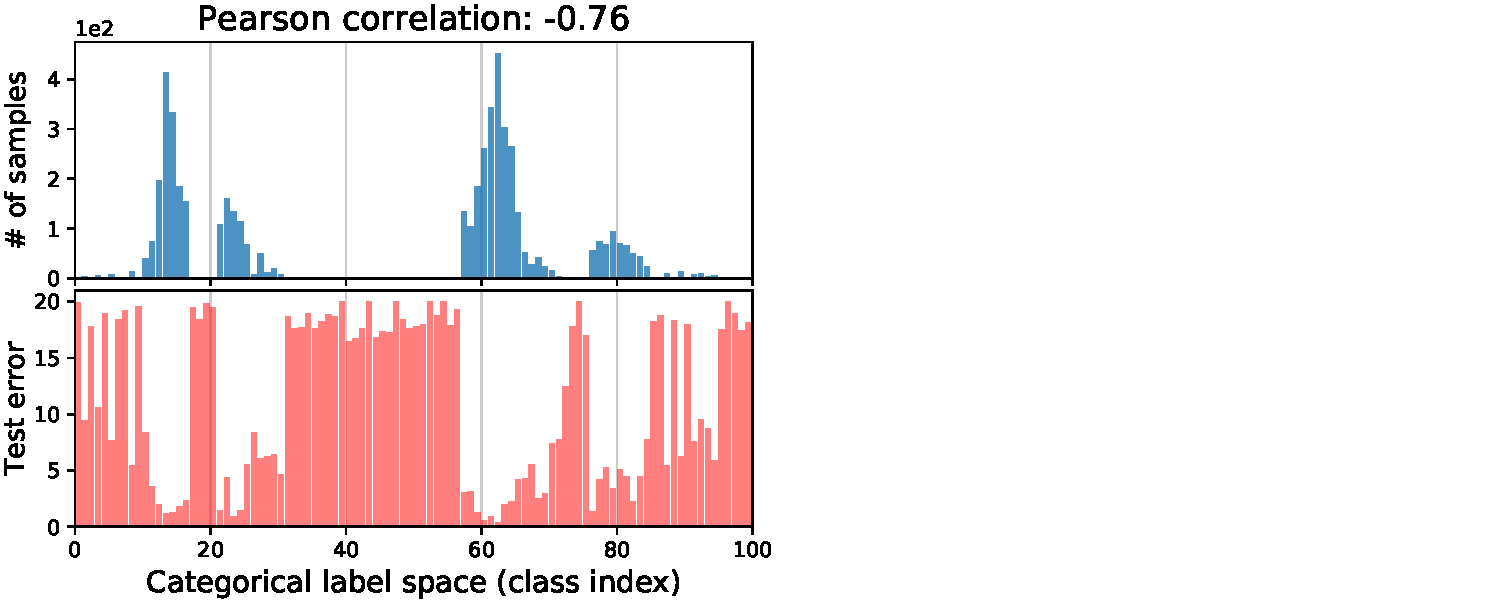
\includegraphics[width=\linewidth]{images/err_motivate_1_left.pdf}
			\caption{Classification}
		\end{subfigure}\hspace{1em}%
		\begin{subfigure}{0.44\textwidth}
			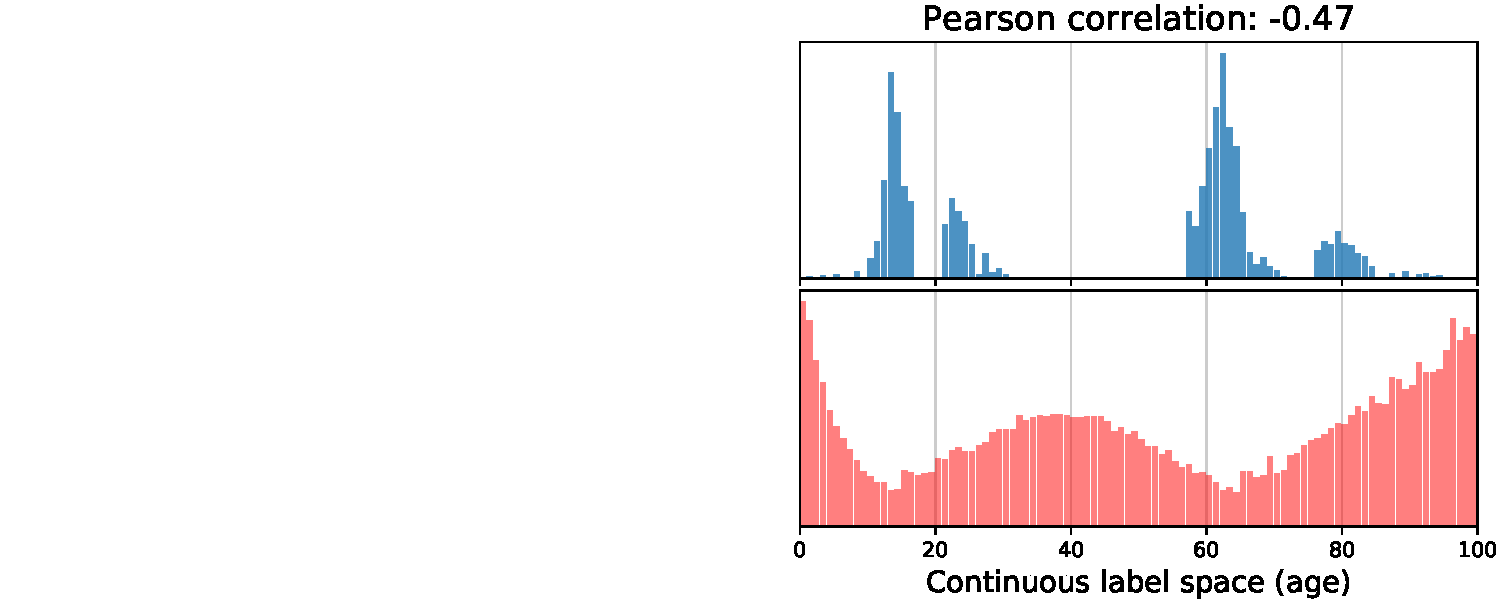
\includegraphics[width=\linewidth]{images/err_motivate_1_right.pdf}
			\caption{Regression}
		\end{subfigure}
		%\caption{}
	\end{figure}
	\footnotesize
	\vspace{-1em}
	\begin{columns}
		\begin{column}{0.5\textwidth}
			\begin{itemize}
				\item Compensating for the imbalance in the empirical label
				density distribution WORKS WELL.
			\end{itemize}
		\end{column}
		\begin{column}{0.5\textwidth}
			\begin{itemize}\setlength\itemsep{0em}
				\item The empirical density does not accurately reflect the imbalance as seen by the model.
				\item Compensating for the imbalance in the empirical label
				density distribution is INACCURATE.
				\item Proposed solution: \textbf{Label distribution smoothing}
			\end{itemize}
		\end{column}
	\end{columns}
	\credit{Image}{yang2021delving}
\end{frame}

\begin{frame}{Label Distribution Smoothing (LDS) - Overview}
	\begin{figure}[h]
		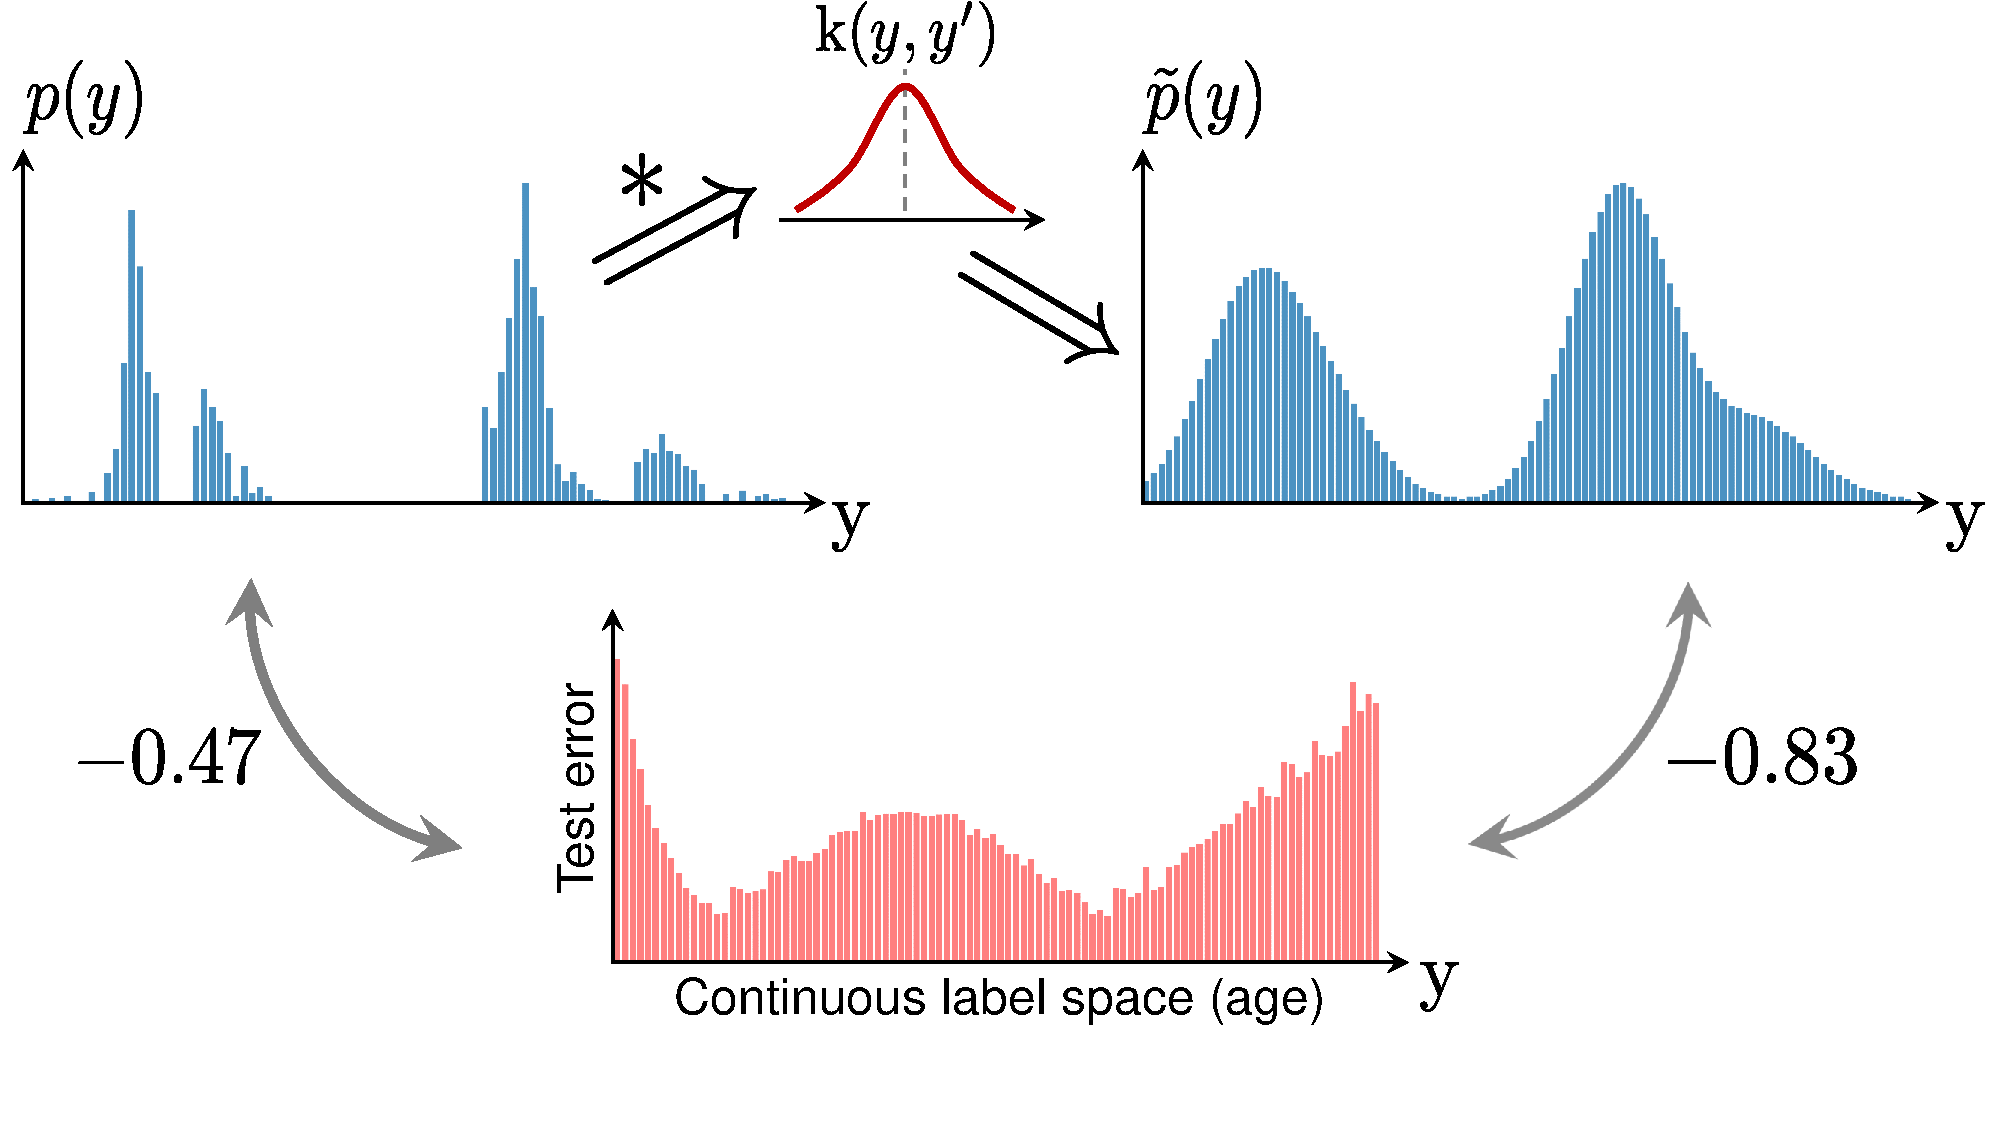
\includegraphics[width=\linewidth]{images/err_motivate_sep.pdf}
		%\caption{}
	\end{figure}
	\credit{Image}{yang2021delving}
\end{frame}